%!TeX program = xelatex
%Do not change
\documentclass[12pt, oneside]{article}
\usepackage{amssymb,amsmath}
\usepackage[margin=1in]{geometry}
\usepackage{textpos}
\usepackage{float}
\usepackage{booktabs}
%\usepackage{color}
\usepackage{graphicx}
\usepackage[inter-unit-product =\cdot]{siunitx}
\let\DeclareUSUnit\DeclareSIUnit
\let\US\SI
\DeclareUSUnit\inch{in}
\DeclareUSUnit\foot{ft}
\DeclareUSUnit\mile{mi}
\DeclareUSUnit\foot{ft}
\DeclareUSUnit\slug{slug}
\DeclareUSUnit\pound{lb}
\DeclareUSUnit\psi{psi}
\DeclareUSUnit\Msi{Msi}
\DeclareUSUnit\ksi{ksi}

\usepackage{tikz}
\usetikzlibrary{positioning}
%\usepackage{tikz-3dplot}
\usepackage{pgfopts}
%\usepackage{wasysym}
\usepackage{stanli}

% You may add the packages you need here
\begin{document}

%TODO change numbers in problems
\begin{textblock*}{4cm}(-1.7cm,-2.3cm)
\noindent {\scriptsize AE333 Fall 2020}
\end{textblock*}

%Do not modify other than putting your name where stated
\begin{textblock*}{8cm}(12.5cm,-1cm)
\noindent {Name: }
\end{textblock*}
%Do not modify other than typing your acknowledgement where stated
\begin{textblock*}{13.5cm}(-1.7cm,-1.8cm)
%\noindent \textit{\footnotesize Acknowledgement: Your acknowledgement for collaboration and other sources goes here. }
\end{textblock*}

\vspace{1cm}

%Do not modify other than typing the homework number after #
\begin{center}
\textbf{\Large Homework 10}

\textbf{Due 3 December 2020}
\end{center}

\begin{enumerate}
	\item %4-92
		Determine the maximum normal stress developed in the bar when it is subjected to a tension of $P = 	\US{4 }{kip} $
		\begin{figure}[H]
			\centering
			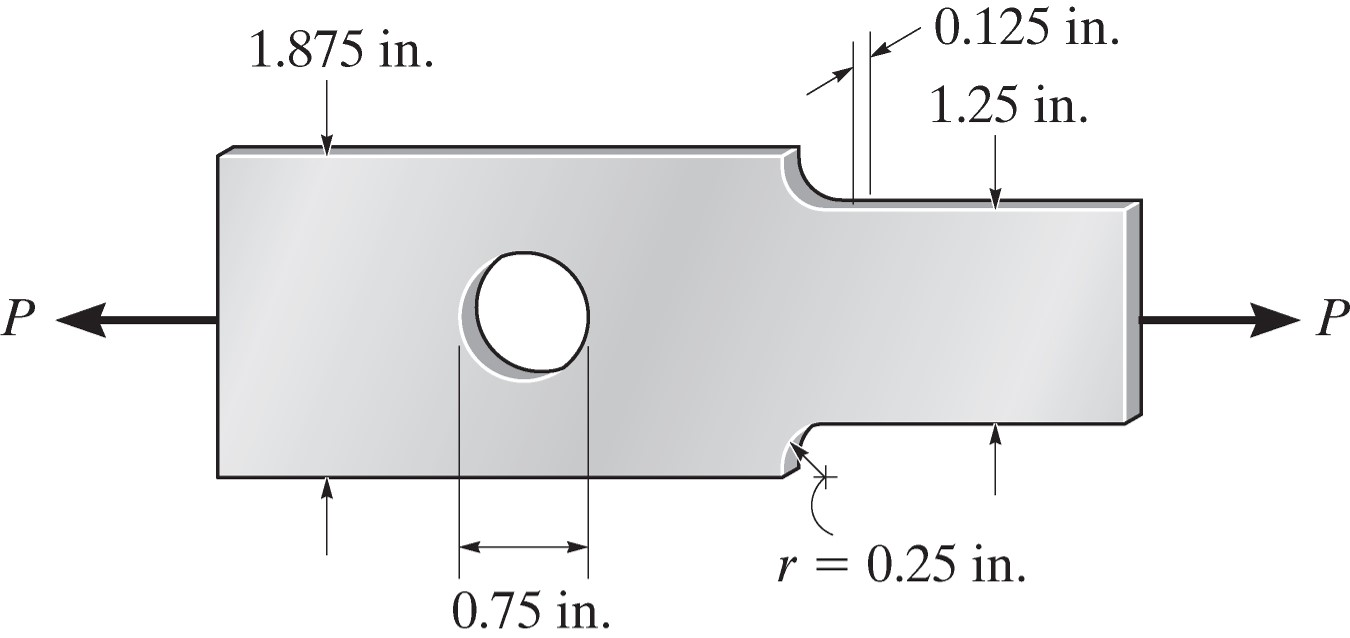
\includegraphics[width=0.8\linewidth]{4-92}
		\end{figure}

	\item %4-90
		The A-36 steel plate has a thickness of $ 	\SI{12 }{mm}  $.
		If $\sigma_{allow} = 	\SI{135 }{MPa} $, determine the maximum axial load, $P$ that it can support.
		\begin{figure}[H]
			\centering
			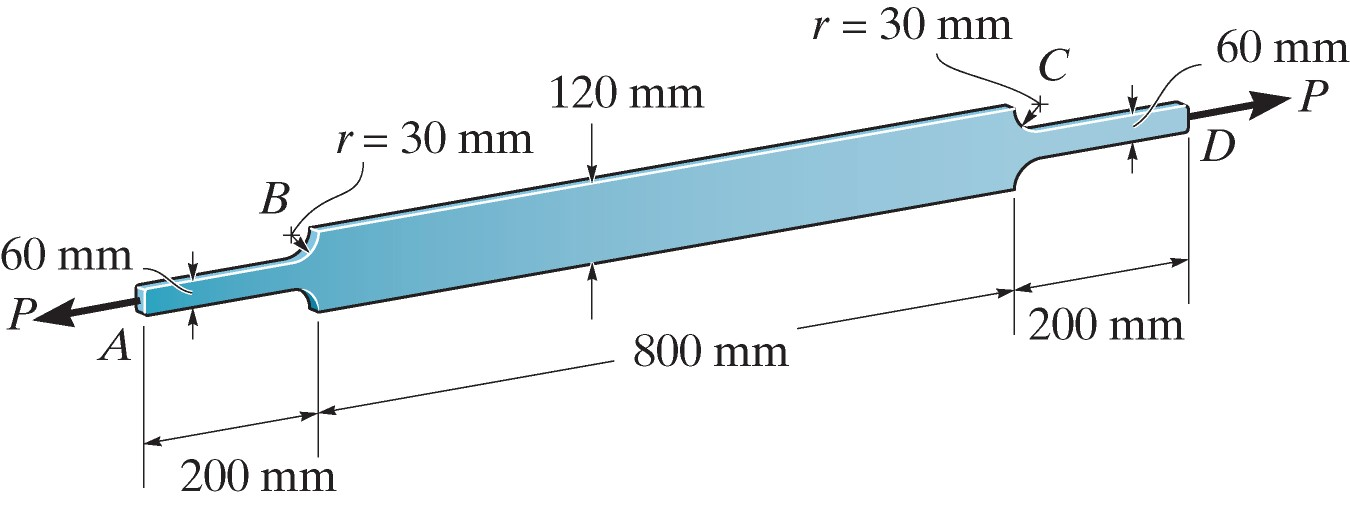
\includegraphics[width=0.6\linewidth]{4-90}
		\end{figure}
		\newpage

	\item %5-124
		The shaft is fixed to the wal at $A$ and is subjected to the torques shown.
		Find the maximum shear stress in the shaft.
		A fillet weld having a radius of $ 	\SI{2.75 }{mm}  $ is used to connect the shafts at $B$
		\begin{figure}[H]
			\centering
			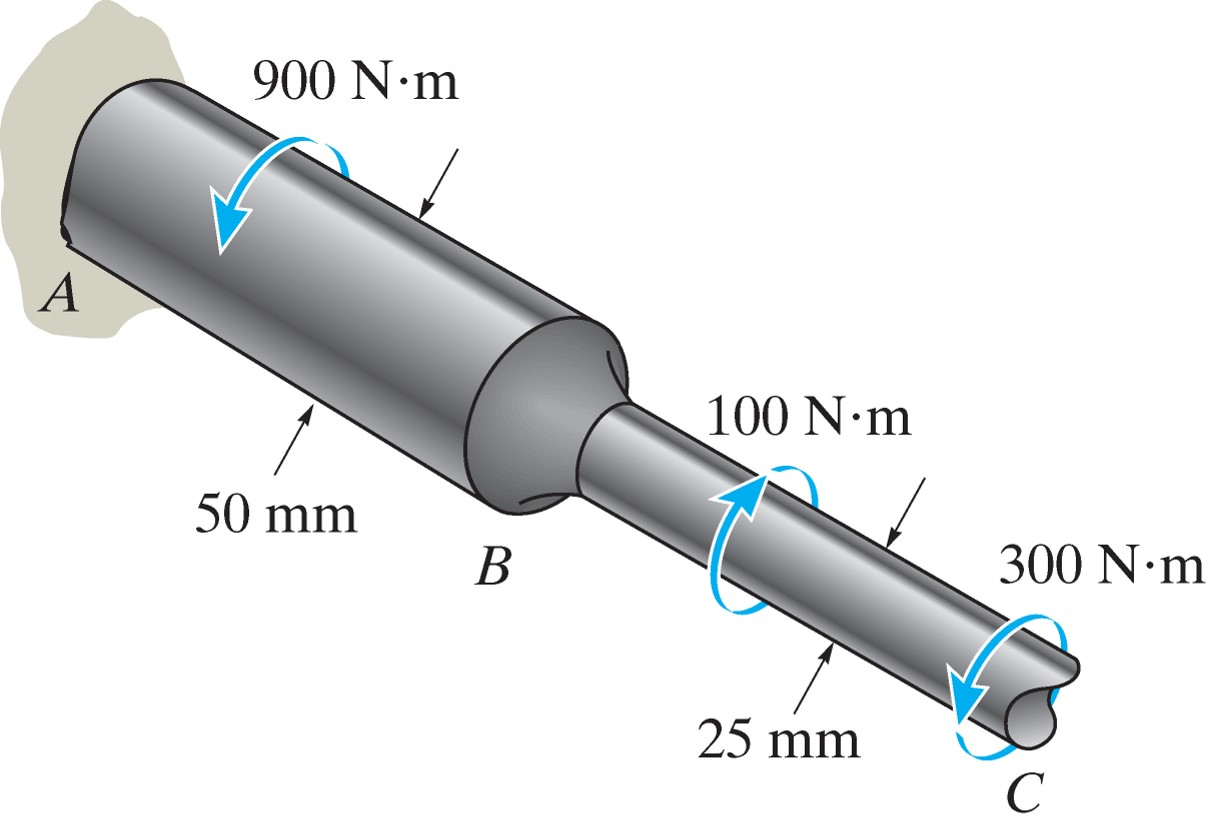
\includegraphics[width=0.6\linewidth]{5-124}
		\end{figure}

	\item %6-155
		If the radius of each notch on the plate is $ 	\SI{10 }{mm}  $ find the largest moment $M$ that can be applied.
		The maximum allowable bending stress is $\sigma_{allow} = 	\SI{190}{MPa} $
		\begin{figure}[H]
			\centering
			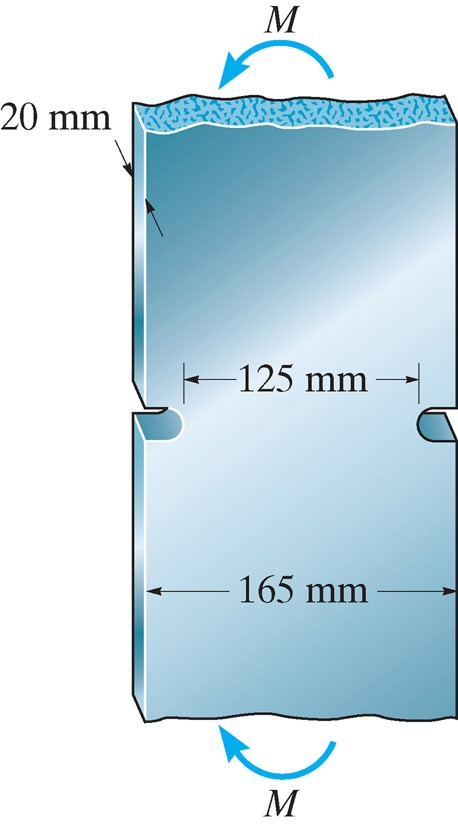
\includegraphics[width=0.3\linewidth]{6-155}
		\end{figure}
		\newpage

	\item %13-14
		The W8 x 67 flange 2014-T6 aluminum column can be assumed to be fixed at its base and pinned at its top.
		Find the largest axial force, $P$, that can be applied without causing buckling.
		\begin{figure}[H]
			\centering
			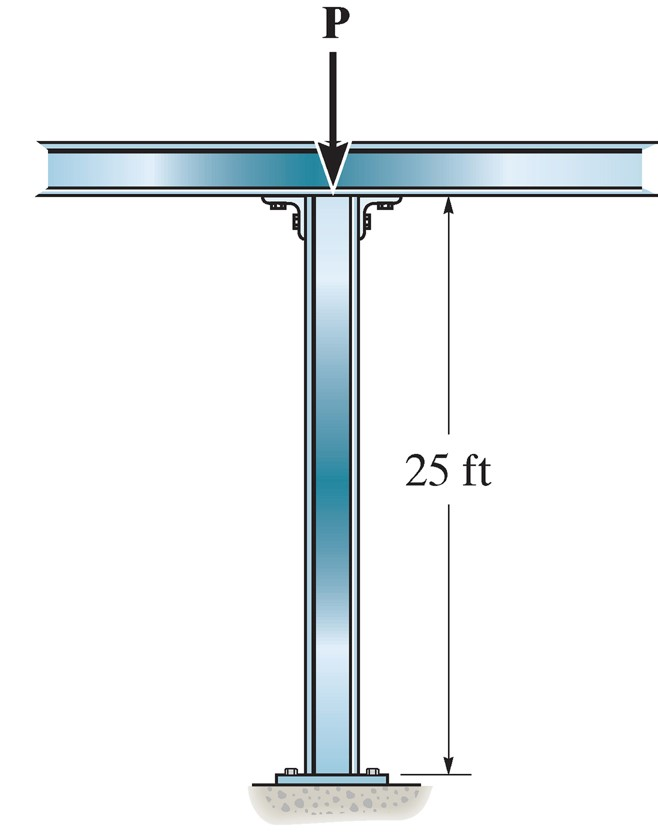
\includegraphics[width=0.6\linewidth]{13-14}
			\caption{13-14}%
			\label{fig:13-14}
		\end{figure}

	\item %13-15
		Solve the previous problem assuming that it is fixed at its base and free at its top

	\item
		Repeat the previous problems assuming that it is fixed at both the base and top.
		Which of these cases is the best for buckling, which is the worst?

\end{enumerate}
\end{document}
